\section{Preliminaries}

The User Space component is a server process that provides the web service. Its main tasks are to mediate the services of the translation memory and to reflect all the users' GUI activity and make the user's work persistent on the server and available always in the same state she finished her work.

The User Space is a Java Servlet which is run using the \emph{Jetty WebServer}. All of the User Space code is implemented Java. It uses \emph{Hibernate} object-relational mapping library. The same \emph{PostgreSQL} database as in the TM Core is used. The in-memory \emph{hsqldb} database is used for the unit testing.

Because the TM Core is a separate module it is also linked as dependency to the User Space, but they run together as one process in one Java Virtual Machine. Their communication is done by invoking the core methods returning objects of share classes.

\section{Architecture}

To make the whole project as clear as possible we try to use as most as possible from the shared classes and prevent using the User Space specific classes. If some additional functionality is required and cannot be incorporated into the shared classes, mostly the database and core calls, we wrap the shared classes into distinct User Space classes.

The server class which processes the calls on the first level contains the {\it Session} objects. These objects processes the calls with association the the particular logged in users. These two classes are not a part of the shared classes set.

The session class contains an object representing the user (a wrapper for the shared class). Hash tables of active documents is there to access  them quickly. Both the document objects and translation results objects (which collect the source chunk, translation suggestion and the actual user's translation) are wrappers for the shared classes. Anyway, the inner shared objects are used for communication with other components.

The more basic level than the translation result uses exactly the shared classes structure.

\section{Functionality overview}

The User Space services are available via the RPC calls from the client side. During the run of the server there exist one instance of the server class. The main task of the sever class is to process the calls from the clients -- which in fact means pass the calls further to the particular sessions and manage the sessions themselves. There is a method for every single operation that is possible to happen in the client.

After a user logs in, a Session object is created. It contains a unique session ID the client uses for authentication of its calls. A session object contains information about the user -- the user's settings and \todo{this is not true}a list of the documents owned by the user, and hash tables of documents and chunks which are currently in use. When the user is logged in all of the call processing is happening in the session class.

Until the user does not explicitly request a document, only basic information about the document remains loaded into memory (basic facts about the movie, time of last changes of the document). Only if he opens the document for editing, all the document chunks with the translation suggestions and already finished users translations are loaded. Anyway, if the list of owned documents is queried, empty documents arrive to the client no matter if the documents are loaded in the User Space.

There is also a thread running in the server that checks the time how long the sessions are opened without any users action. If this time exceeds the predefined session time out limit, either a short time for common sessions or a very long time for permanent sessions, the session is terminated. The another situations when a session is terminated is when the user logs in despite has he already owns a session or explicitly logs out. When a session ends, basic information about the session is written to database (user, start time, end time) to enable us to compute statistics about using the application later.

\begin{figure}
\begin{center}
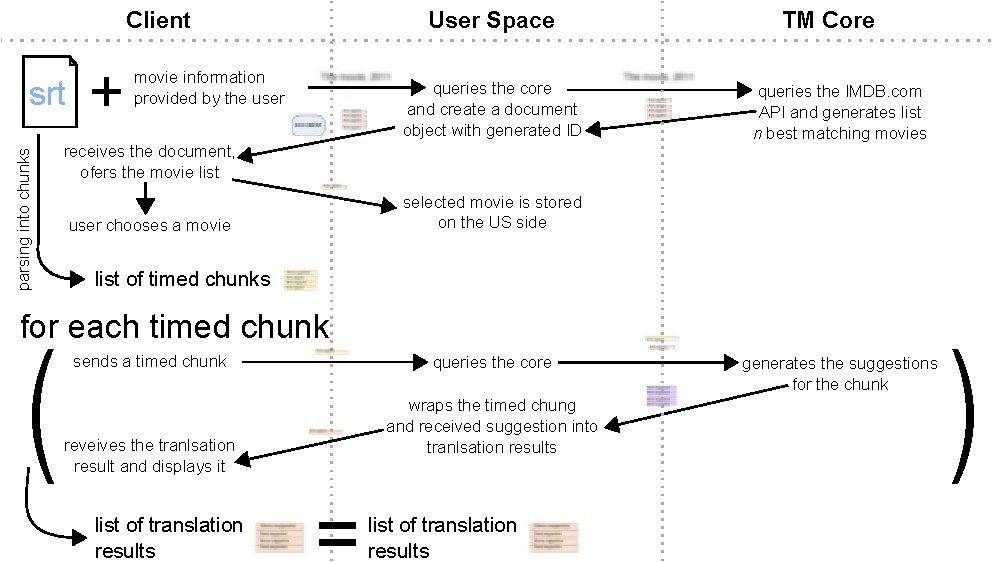
\includegraphics{figures/creating_document.pdf}
\end{center}
\caption{Structure of component communication during a new document creation}
\end{figure}

When a new document is created, the User Space receives a basic information about the movie first. Based on that it creates a Document object and saves it to the database immediately, to receive a unique  database ID which is the used as a document identifier in all other calls. The core is called at this moment to provide a list of possible movies with best matching title and year of production together with genre tags obtained from the Freebase knowledge base. The user is then supposed to choose one or none of the suggested movies. This information is used by the User Space at the moment the core is queried for the translation suggestions.

When a new document is created, the client application starts to send the batches of chunks which are supposed to be translated. When the User Space receives such call, it queries the TM Core for the translation suggestion and adds the chunks to the list list chunks which the appropriate document consists of. Once the suggestion are generated they are thrown away immediately. Keeping a copy of them in memory during runtime and saving them to the database would increase massively the memory requirement and the database size, which can be easily avoided. This also means that when the client queries the saved translation results it will receive them without the translation suggestions. In such case the suggestions are provided by on demand calls per chunk. \todo{refer to the place in GUI documentation}

User Space also provides feedback to the translation memory. A list of new translation the users have produced can be generated together with information which translation pair they used to post-edited is provided to the Data Import module which adds the new translation to the translation memory and use the data also for training the scoring of the suggestions. \todo{Add a reference to the place this is described}

Export of the subtitle files is also solved in the User Space. It is described in more detail in section \ref{sec:export}.

\section{Implementation Details}
\subsection{The Data Types Overview}

The User Space uses the shared data types used thorough the application or the wrapper of such classes. A brief overview of the used classes and their role in the User Space follows. (Prefix US means User Space.)

\begin{itemize}
\item {\tt FilmtitBackendServer}  -- The class is the Java Servlet whose public methods are invoked by the RPC calls. Its main task is to mediate the calls to concrete opened sessions and take care of users login. A thread checking if there some sessions without activity for a long time and termites the non-active sessions is run the server class.

\item {\tt Session} -- The class represents a running session. There is exactly one session object for one logged in user, it is actually the Session class which process the client calls. It contains hash tables of actively edited documents to make them quickly accessible by their IDs. During the existence of a session object all the client side operations are stored just in the memory and saved immediately to the database. When the session ends -- either by the user logging out or by exceeding the maximum time without a user action -- a record about the session is stored to database -- id of the user that owned the session, its start time and end time. This is intended as an activity log from which further statistics can be inferred.

\item {\tt USUser} -- This class is a wrapper of the shared User class. During the existence of the session its used as a provider of the documents owned by the user. It is also used for storing the settings of the user. In advance to the shared class a set of documents which has been left opened when the last user's session was terminated is also stored in the class which is used at the time a new session is created. 

\item {\tt USDocument} -- The class is a wrapper of the shared {\tt Document} class. A {\tt USDocument} object represents a subtitle file with additional information about the movie it belongs to. Its content is supposed to be a mirror image of the Document object on the client side. It contains a list of Translation Results representing the actual subtitle chunks if the document is loaded to be edited. It is not connected to the translation results by the database mapping to make it easy to send the list user's documents without the actual content.

\item {\tt USTranslationResult} -- It is a wrapper for the shared {\tt TranlsationResult} class. The class congregates the original subtitle chunk, its timing, the translation suggested by translation memory and the result of the user activity -- the user's translation which translation suggestion she has chosen. It is the class where the actual translation is being done. Despite a user can delete the document he is working all the translation results are kept in the database to provide a  feed back to the translation memory.

\item {\tt Emailer} -- A class used for sending email from the application. It is used as a confirmation of user registration and also when the user forgets his password and requires sending a new one via email.

\end{itemize}

There are also two third-party classes included in the User Space source code. It is the {\tt IdGenerator} class which generates id sessions (distributed under the {\it Apache License, Version 2.0}) and the {\tt BCrypt} class which ensures hashing the passwords before we store them in the database (distributed under {\it BSD licence}).

The {\tt SubtitleDownloadServlet} class responsible for exporting the subtitle files is described in section \ref{sec:export}. Details concerning the user registration, login and using open ID are discussed in more detail is section \ref{subsec:simple_login} in the GUI chapter. Details about handling the communication with the client are covered in section \ref{sec:communication} of the GUI chapter.

\subsection{Database Mapping}

As was mentioned many times before, the User Space mirrors all the client operations and make them persistent on the server side. The persistence ensured by saving the data to the database. The exist many sophisticated tool for Java to ensure the data persistence, e.g. \emph{Java Persistence API} framework which or some frameworks working on the higher level of abstraction as \emph{Spring Data Framework}. Since only very basic database operations are required during the run of the User Space -- loading and saving of the raw Java object -- only a object relational mapping is library used, namely the \emph{Hibernate}.

The core also uses Hibernate for mapping the {\tt MediaSource} class (gathering information about movie). User Space shares the mapping of such class and uses a class extended from the core class to manage the database transactions.

The mapping just reflects the data properties of classes. If the class is a wrapper of a shared class the getters and setters of the properties are bind to the wrapped objects properties.

As was told before, the mapping of {\tt USDocument} does not include the list of Translation Results the document contains in order to be able to send the documents both with and without the translation results. It would be also possible to use the lazy Hibernate collection mapping, but it would cause problem at the time the object serialized.

\subsection{Providing Feedback to the Translation Memory}

In order to be able provide a feedback to the translation memory and take advantage of the translator work for improving of the translation memory, the implementation of deleting a document a selecting of the media source needs to be done not in a straightforward way. Handling this requirements is described in following paragraphs.

The User Space and the Translation Memory Core use the same database table for the media source (representing the movie or the TV show the subtitles are from). When the user creates a document she is required to enter the title of the movie she is about to translate. After that the {\it Freebase} service is queried for the movies and TV shows possible having such title and a list of this matches is provided to the user to choose from. After the user chooses the media source, the media source object is sent back to the User Space. Then the search in the database table is done. If there is a record with the same title and the release year, its data (genres and thumbnails URL) are updated, if it is a completely new media source, it is saved to the table.

The reason for doing it is not to have duplicate media sources in the database and also the fact that the meta data of the movie should be available to the Data Import module when the feedback to the translation memory is provided.

Another thing to be mentioned here is handling the document deletion. When the user clicks on the delete button in the interface, the document is marked to be deleted in the User Space and is removed from the list of documents owned  by the user and from the list of the documents that has been loaded during a session. From that time the document is not available for the user. After dealing with this a thread is run that deals with the translation results the document consists of. All the translation results that has already provided the feedback to the translation memory are deleted from the database. If the document is empty after this step, it is delete too.

Providing the feedback itself is done by a static method of the {\tt USTranslsationResult} class. This method returns all the translation results what have not been used for feedback before (have {\tt hasSentFeedback} flag set to false. The translation results are provided with a reference they belong to which allows resolve the media source later. If the translation results are form a document that has been flagged as ready to be deleted, both the translation results and the document are delete. Otherwise just the flag informing about having provided the feedback is set.

\section{Exporting Subtitle Files}
\label{sec:export}

TODO \todo{Write it}

